\section{Bilancio di esercizio}
\subsection{Contabilità generale( Co. Ge)}

Insieme dei procedimenti informativi che utilizza lo
strumento contabile e il metodo della partita doppia

Ha lo scopo di rilevare i flussi finanziari e dei correlativi flussi economici.

\subsection{Il metodo della partita doppia}

\begin{itemize}
    \item istituire: fissare l'oggetto e la denominazione di un conto
    \item aprire o accendere: effettuare la prima registrazione
    \item chiudere: tirare la somma algebrica e scrivere nella sezione con totale minore, il valore per arrivare in pari fra le cose postive e quelle negative
    \item addebitare: iscrivere una variazione di conto in dare
    \item accreditare: iscrivere una variazione di conto in avere
    \item stornare: eliminare da un conto una quantità e trasferirla in un'altro conto
    \item riepilogare: trasferire il contenuto di più conti in uno di sintesi
    \item funzionmento antitetico dei conti(conti in sezioni diverse hanno segno opposto)
    \item duplicità dell'aspetto di osservazione
        \begin{itemize}
            \item ogni fatto dever essere osservato secondo un dulice aspetto(origine e derivato)
            \item di conseguenza si avranno conti accesi all'aspetto originario e conti accesi all'aspetto derivato
        \end{itemize}
    \item funzionamento antitetico delle classi di conti
\end{itemize}


Da queste regole deriva che:
\begin{itemize}
    \item la somma degli importi in dare di tutti i conti è uguale alla somma in avere di tutti i conti
    \item la somma dei saldi in dare di tutti i conti è uguale alla somma dei saldi in avere di tutti i conti
    \item la somma algebrica dei saldi in una parte qualsiasi dei conti del mastro è uguale e di segno opposto alla somma algebrica dei saldi della rimannente parte dei conti
\end{itemize}

\subsection{Metodo della partita doppia: rilevazione dei fatti di gestione}
\begin{itemize}
    \item valori finanziari
        \begin{itemize}
            \item denaro e valori assimilati
            \item crediti e debiti di funzionamento
            \item crediti e debiti di finanziamento
        \end{itemize}
    \item valori economici
        \begin{itemize}
            \item reddito(enttrate - uscite)
            \item capitale
        \end{itemize}
\end{itemize}

I valori finanziari in prevalenza si riferiscono all'aspetto
originario mentre i valori economici si riferiscono
all'aspetto derivato di osservazione.

Le classi di conto sono due: conti finanziar(aspetto originarioi) e conti economici(aspetto derivato).


\subsubsection{Conti finanziari}
Accolgono in dare le variazioni positive e in avere le variazioni negative.

\subsubsection{Conti economici}
Accolgono in dare le variazioni negative e in avere le variazioni positive.

\subsection{Il modello del bilancio}
Il bilancio di esercizio ha lo scopo di determianre e di rappresentare le condizioni di equilibrio
economico, finaziario e patrimoniale dell'azienda.

Offre infromazioni sul risultato economico di un singolo periodo(31/12).


Il risultato economico di periodo si forma mediante le operazioni di gestione dell'attività.

Serve a misurare il variare della ricchezza di un periodo.


Il risultato economico globale è il risultato conseguito durante tutto il periodo di vita dell'azienda(sommo tutti i risultati di periodo).

\begin{figure}[H]
    \centering
    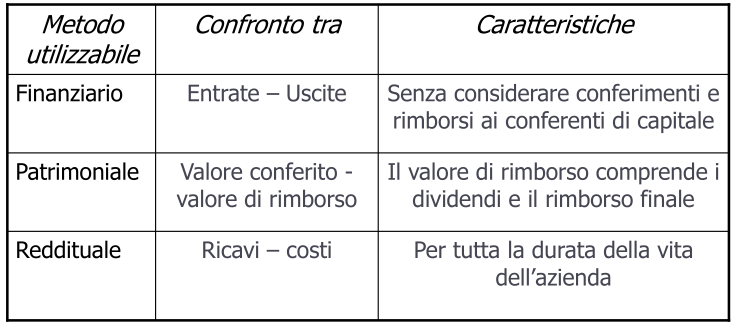
\includegraphics[width=0.7\linewidth]{2/img/Screenshot from 2022-07-06 15-27-34.png}
\end{figure}

\subsection{Costo di acquisizione e costo di utilizzazione}

Il costo di acquisizione è il costo speso per un certo fattore produttivo(ferro, macchinario, ecc).


Il costo di utilizzazione è il valore dei fattori produttivi che vengono usati nella realizzazione
di un prodotto o di un servizio che hanno generato un ricavo.


La differenza tra costo di acquisizione(dinamica monetaria) e costo di utilizzo(dinamica economica)
 di un fattore produttivo a fecondità ripetuta rappresenta il valore residuo del fattore produttivo, il che implica che ci siano
 ancora operazioni possibili con un certo asset.

 \subsection{Ammortamento}
 La quota di ammortamento rappresenta il valore che può essere fatto partecipare in componente negativa 
 al risultato economico di periodo.

 In questo modo i fattori produttivi vengono suddivisi sul periodo nel quale vengono utilizati.

 \subsection{Il principio di competenza}
 Sono di competenza di un periodo i costi ed i ricavi dei processi compiuti:
 \begin{itemize}
    \item conclusi con il conseguimento dei ricavi
    \item con la condizione che nello stesso periodo si sia effettuata anche la prestazione
 \end{itemize}

 \subsection{Principio di prudenza}
 Il risultato economico di periodo è un valore astratto e non implica le disponibilità
 di cassa dell'azienda.

 Per trasferire la ricchezza prodotta ai conferenti di capitale di rischio senza che si
 svuotino le casse della gestione si devono considerare le perdite anche se solo temute e
 non considerare i ricavi se solo sperati.

 \subsection{Capitale di funzionamento}

 Al termine di un periodo rimangono fattori produttivi:
 \begin{itemize}
    \item generici(denaro, risorse finanziarie)
    \item specifici(prodotti da usare, cicli produttivi da terminare e prodotti da vendere)
 \end{itemize}

 \subsection{Il modello del bilancio}
 il modello economico finanziario consente di misurare e rappresentare l'economicità(equilibrio economico, patrimoniale e finaziario),
 rispettando delle condizioni:
 \begin{itemize}
    \item efficacia(raggiungere gli obiettivi)
    \item efficienza(minor risorse usate per l'obiettivo)
 \end{itemize}

 Queste cose vengono analizzate dal modello del bilancio.


 \begin{itemize}
    \item Oggetto dedl bilancio
        \begin{itemize}
            \item insieme dei valori economici e finanziari che derivano dalla gestione e rappresentano variazioni delle risorse
        \end{itemize}
    \item finalità del bilancio
        \begin{itemize}
            \item rappresentazione chiara, veritiera e corretta della situazione patrimoniale e finanziaria della società e del risultato economico.
        \end{itemize}
    \item prospetti fondamentali
        \begin{itemize}
            \item stato patrimoniale
            \item conto economico
            \item (rendiconto finaziario)
        \end{itemize}
 \end{itemize}

 \subsection{Stato patrimoniale}
 Descrive la situazione patrimoniale in certo istante.

 \begin{itemize}
    \item valore monetario misurabile = \textbf{attività}
    \item diritti vantati da terzi = \textbf{passività}
    \item diritti vantati dai soci = \textbf{patrimonio netto}
 \end{itemize}

 Il valore attività è forato dalla somma del patrimonio netto e delle passività.

 \subsubsection{Struttura sintetica}
 \begin{figure}[H]
    \centering
    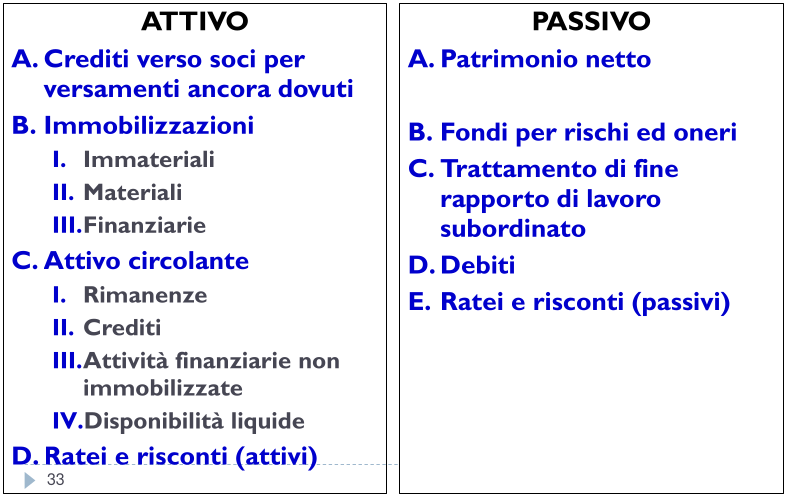
\includegraphics[width=0.7\linewidth]{2/img/Screenshot from 2022-07-06 16-07-29.png}
\end{figure}

\subsection{Conto economico}

Sintesi dei flussi di natira economica(ricavi e costi) che interessano l'impresa in un certo intervallo temporale.

Evidenzia la progressiva formazione del risultato economico di periodo.

\subsubsection{Struttura sintetica}
\begin{figure}[H]
    \centering
    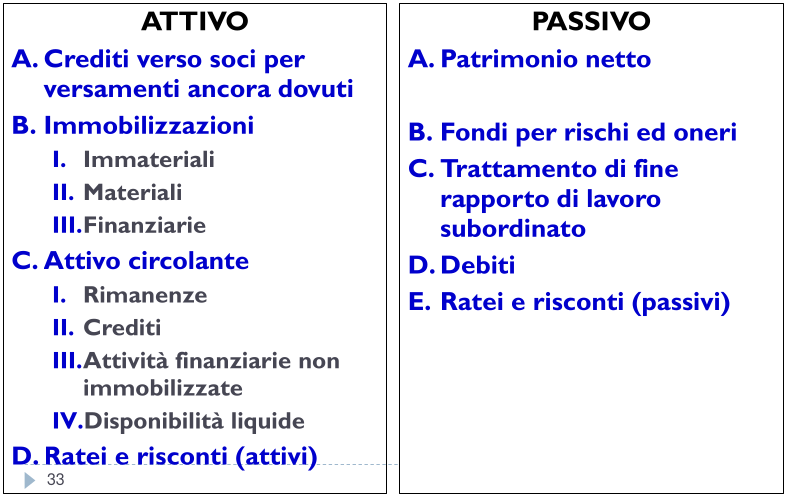
\includegraphics[width=0.7\linewidth]{2/img/Screenshot from 2022-07-06 16-07-29.png}
\end{figure}
